\documentclass[a4paper,12pt,titlepage]{article}
\usepackage[left=2cm,top=3cm,right=2cm,bottom=1cm,head=2.0cm,includefoot]{geometry}
\usepackage[spanish,activeacute]{babel}
\usepackage{fancyhdr}
\usepackage{graphicx}

\title{\textbf{Elevadores H\'ercules S.A.}}
\author{\textbf{Grupo B1}}

\begin{document}

\pagestyle{fancy}
\chead{Grupo B1}
\lhead{
\includegraphics[width=1.7cm]{./logo1.png}}
\lfoot{71.12 - Estructura de las Organizaciones}
\rfoot{$1^{er}$ Cuatrimestre 2011}
\maketitle
\tableofcontents
\newpage

%documento

\section{\underline{Enunciado}}
Elevadores H\'ercules S.A., establecida en Buenos Aires en 1919 como una oficina de
contratistas, se desarrollo al punto de transformarse en una de las compa\~n\'ias m\'as
importantes del mundo. En 1966, la compa\~n\'ia produc\'ia 1650 elevadores y en 1974
lleg\'o a 7.850 unidades, inclusive escaleras mec\'anicas. Aunque su planta principal est\'a
ubicada en Buenos Aires, tiene oficinas comerciales en las 18 ciudades m\'as
importantes del pa\'is participando con m\'as del 60\% del mercado nacional. A partir de
1970 el n\'umero de edificios comenz\'o a aumentar considerablemente. Los pedidos de
los clientes tend\'ian a alcanzar l\'imites que sobrepasaban la capacidad de producci\'on
de la f\'abrica. Los atrasos en la entrega de pedidos llegaron al punto de provocar serios
conflictos entre los departamentos de ventas y producci\'on.\\
En funci\'on de lo anterior, la alta direcci\'on de la compa\~n\'ia decidi\'o perfeccionar el
sistema de planeamiento y control de la f\'abrica.\\ \\
\textbf{Principales caracter\'isticas del sistema de producci\'on:}\\
La producci\'on de elevadores requiere cerca de 6.000 diferentes grupos de piezas de
varios tipos o medidas y aproximadamente 12.000 \'items de stock. La mayor\'ia de los
fabricantes depende de sus proveedores para piezas especializadas como por ejemplo
motores el\'ectricos, cabinas, relees de contacto, gu\'ias, puertas metalizas y cerraduras.
Al contrario de esto, elevadores H\'ercules S.A. tiene la directriz de ser autosuficiente y
producir todas las piezas que utiliza. De esto resulta que la empresa tiene una
producci\'on bastante diversificada, que no es com\'un en su ramo y que da origen a un
complejo sistema de planeamiento y control de la producci\'on.\\
La producci\'on de elevadores no puede seguir un plan general, por que los pedidos
var\'ian considerablemente de acuerdo a las necesidades de los edificios en
construcci\'on. Apenas algunas partes de los elevadores H\'ercules son Standard y
producidas para stock, como por ejemplo: correderas-gu\'ias, gu\'ias de puerta,
cerradores, motores y conjuntos de motores generadores, relees de contacto y botones
de llamada. El planeamiento de producci\'on esta dificultado tambi\'en por el desarrollo
tecnol\'ogico de la construcci\'on de diferentes tipos de lugares, dependiendo por eso de
condiciones que dif\'icilmente se pueden prever.\\
El equipo de producci\'on y montaje de elevadores estaba dividido en 4 grupos
generales, de acuerdo con la secuencia a ser seguida en la entrega de partes,
conforme al siguiente esquema:\\
\begin{itemize}
 \item[-] GRUPO \#1\\
Modelo soporte para la cabina, gu\'ias, correderas, barras, amortiguadores, base,
maquina y polea de desvi\'o.
\item[-] GRUPO \#2\\
Tablero de comando
\item[-] GRUPO \#3\\
Armaz\'on de cabina, Contrapesos, paragolpes, plataforma, cabina y cables de acero.
\item[-] GRUPO \#4\\
Puertas de lobby, visores, cerraduras, botones de llamada y otros detalles necesarios
para que complete el montaje en el edificio.
\end{itemize}

La producci\'on de la f\'abrica estaba organizada a trav\'es de las siguientes secciones:
\begin{enumerate}
 \item Maquinas operativas, tornos, plegadoras, perforadoras, rectificadoras
 \item Estampado
 \item Montaje de maquinas
 \item Montaje de motores
 \item Montaje de aparatos electricos
 \item Montaje y conexi\'on de cuadros de comando
 \item Carpinter\'ia, fabricaci\'on de contrapesos, cabinas y puertas de acero.
 \item Carpintero, cabinas, puertas y plataformas de madera
 \item Pintura y galvanoplastia
\end{enumerate}

En 1970, el planeamiento de producci\'on de elevadores H\'ercules S.A. era un simple
proceso basado en reportes mensuales de campo del departamento t\'ecnico,
encargado del montaje de los elevadores, formado por varios grupos de empleados
especializados. Cada grupo era responsable por el control de una cierta \'area de la
ciudad. El jefe de grupo visitaba peri\'odicamente a varios clientes de su localidad y
estimaba futuras necesidades. Completaba un formulario de ``avances del mes'' donde
volcaba los avances de cada obra indicando el grado de avance de la construcci\'on y
estableciendo los programas de entrega de acuerdo con los cuatro grupos generales
del proceso de producci\'on y montaje ya mencionados. Una vez que el formulario se
completaba, le era entregado al planeador de la producci\'on, un antiguo supervisor que,
en 1942, se convirti\'o en asistente del departamento de producci\'on a fin de controlar el
proceso de planeamiento de la compa\~n\'ia.\\
A partir de los formularios de ``avances del mes'' recibidos por todas las \'areas, el
planeador elaboraba el programa de producci\'on para todas las partes a ser producidas
de acuerdo a la secuencia num\'erica indicada por el departamento de ventas y que
obedec\'ia al orden de entrada de los pedidos de los clientes. El planeador recib\'ia
tambi\'en las copias de ``orden de fabricaci\'on individual'' realizadas por el departamento
de ingenier\'ia, conteniendo las especificaciones necesarias para producir cada
elevador.\\
En la \'epoca en que la cantidad de elevadores producidos era relativamente baja en
relaci\'on con la capacidad de producci\'on de la fabrica, el sistema de planeamiento
descrito, probo ser simple y eficiente y pod\'ia ser f\'acilmente controlado por el planeador
y por los jefes de secci\'on que en conjunto programaban la producci\'on, determinando
cantidades y especificaciones, pidiendo materiales a ser producidos por la fundici\'on, de
oficinas o del pa\~nol.\\
Los reportes mensuales de los grupos de campo eran suficientes para dar al planeador
las informaciones en cuanto a las necesidades futuras de los edificios en construcci\'on y
por lo tanto, esclarecer las prioridades de producci\'on.\\
Entretanto a partir de 1970, el n\'umero de construcciones comenz\'o a aumentar. Los
retrasos en las entregas de elevadores hicieron que los jefes de campo fijasen los
plazos de entrega muy anticipados en sus informes mensuales. Con eso las
informaciones recibidas por el programador, fueron perdiendo parte de su valor como
base para la programaci\'on. Ocurri\'o tambi\'en que ni el planeador ni los jefes de secci\'on
de producci\'on eran avisados cuando un edificio ten\'ia sus obras paralizadas, haciendo
que fuese mantenido el stock de sus correspondientes semielaborados. Este
desperdicio agravaba todav\'ia mas la situaci\'on de los atrasos provocando graves
reclamos por parte de otros clientes. Teniendo eso en vista, el departamento de ventas
comenz\'o a sugerir alteraciones en las prioridades distintas a las ordenes de
producci\'on, lo que llevo a los empleados a abandonar los m\'etodos de programaci\'on
que hasta entonces hab\'ia sido establecidos por los jefes de grupo, pasando entonces a
trabajar de acuerdo a las ordenes de ventas del departamento respectivo.\\ \\
\textbf{Decisiones}\\
En vista de la situaci\'on, la alta direcci\'on decidi\'o perfeccionar el sistema de
planeamiento y control de la f\'abrica.
Contratar una consultora para que analice el caso y revertir la situaci\'on de esta compa\~n\'ia.

\newpage


\section{\underline{Interpretaci\'on}}

\title \textbf{\underline{Elevadores Hércules S.A.}}

\begin{itemize}
 \item \textbf{Resumen}\\
      Elevadores Hércules S.A. que en sus principios era una oficina contratista ubicada en Buenos Aires tuvo tal desarrollo que se convirtió 
      en una importante fábrica de ascensores. Con el pasar de los años, la demanda de ascensores fue creciendo como resultado del aumento de 
      la construcción de edificios. Los pedidos de los clientes llegaron a sobrepasar la capacidad de producción de la fábrica trayendo como 
      consecuencia el retraso de la entrega del producto y, por ende, el descontento de los clientes. Además, se sumaba que la forma de 
      organizarse de la empresa, que les había funcionado tan bien cuando había una baja demanda, no lograba adaptarse a los nuevos cambios
      empeorando aún más la situación. Se recurrió a una consultora para que estudiara la situación y encontrara una solución a los problemas.
 \item \textbf{Problemas}\\
      Los problemas que se encontraron en este caso son los siguientes:
      \begin{enumerate}
	\item La capacidad productiva no llega a satisfacer la demanda de los clientes. El departamento de ventas se comprometía a entregar el 
	producto en un lapso de tiempo que no podía cumplirse por parte del departamento de producción. Esto provocaba que ambos departamentos
	entren en conflicto.
	\item La fabricación de los ascensores no es Standard. Sólo una pequeña cantidad de piezas eran comunes a todos. El resto de las piezas 
	que componían al ascensor dependía de los requerimientos dados por el cliente.
	\item La falta de organización dentro de la misma empresa. Esto causaba que los planeadores y los jefes de sección no se enteraran cuando 
	un edificio tenía sus obras paradas haciendo que fuese mantenido el stock de sus correspondientes semielaborados. Este era un problema grave 
	ya que se podía aprovechar esos acontecimientos para avanzar en la construcción de ascensores de otros clientes.
      \end{enumerate}

\end{itemize}

\newpage

\section{\underline{Organigrama}}

\begin{center}
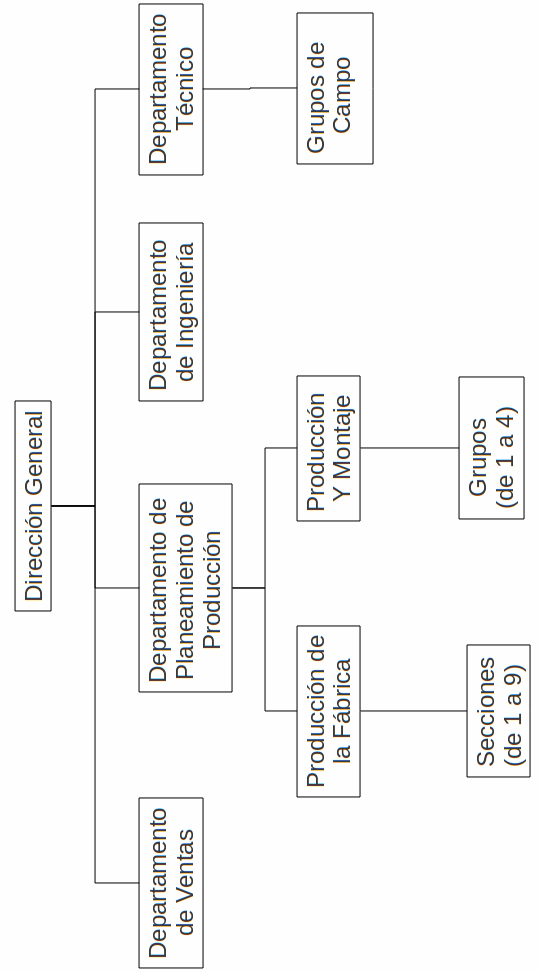
\includegraphics[width=300pt]{./herculesDiag.png}
\end{center}
\newpage

\end{document}
